\documentclass[12pt,a4paper]{article}
\usepackage[margin=2.5cm]{geometry}
\usepackage{amsmath,amssymb,amsthm}
\usepackage{graphicx}
\usepackage{booktabs}

\usepackage{xcolor}
\usepackage[colorlinks=true,linkcolor=blue!60!black,citecolor=blue!60!black,urlcolor=blue!60!black]{hyperref}
\usepackage[numbers,sort&compress]{natbib}
\usepackage{caption}
\captionsetup{font=small,labelfont=bf}

\newtheorem{proposition}{Proposition}
\emergencystretch=2.5em
\newcommand{\kB}{K_{B}}
\newcommand{\kR}{K_{R}}
\newcommand{\etav}{\eta_v}
\newcommand{\etar}{\eta_r}
\newcommand{\etag}{\eta_g}

\title{Optimal Maneuver in Directional Naval Combat:\\
Calibrated Firepower Kernels, Committed-Maneuver Games,\\
and Torpedo Denial in an Auditable World War~II Wargame}

\author{Research Layer of the \emph{Iron Bottom Sound} project\thanks{All
experiments in this paper are fully reproducible from the accompanying
repository: every figure and number is generated by a script in
\texttt{research/experiments/} against a frozen, deterministic rules engine.
The study analyzes a historical board-wargame rules system; it does not
constitute a real-world military decision aid.}}

\date{September 10, 2026}

\begin{document}
\maketitle

\begin{abstract}
Classic surface-fleet tactics---crossing the~T, local fire concentration,
and torpedo threat---are usually justified by doctrine rather than by
game-theoretic analysis.  We develop a two-layer framework that makes these
tactics objects of measurement.  Layer~1 is a directional \emph{firepower
kernel}, a closed-form anisotropic surrogate of a ship's expected gunnery
output, calibrated against the exact probabilistic adjudication of a fully
auditable, deterministic WWII surface-combat rules engine (the open
\emph{Iron Bottom Sound} implementation): on held-out geometry grids the
kernel reproduces engine expected hits with pooled Spearman
$\rho=0.991$ and normalized MAE $5.7\%$ across four ship classes (DD/CL/CA/BB).  Layer~2 embeds the kernel in a two-player
differential game over the reduced relative state $(r,\alpha_B,\alpha_R)$.
We first prove---and verify numerically to machine precision---a
\emph{degeneracy proposition}: with simultaneous moves, identical
instantaneous capabilities, and full observability, the stationary value
collapses to the instantaneous fire differential, so positional maneuvering
has zero equilibrium value.  Maneuvering acquires value only under order
commitment; we therefore solve the committed-maneuver (open-loop) minimax
over a library of sealed battle plans and map tactical regimes over speed
and gun-range ratios.  Speed advantage is found to act
through the reachable tactical set alone: at equal gun range the faster
committed duelist is systematically \emph{worse} off under a pure
fire-differential objective, and speed acquires value only in combination
with a range advantage.
Counterfactual torpedo analysis implements the best-response definition of
maneuver denial.  In the low-direct-hit regime the denial value is exactly
zero---with a measured mechanism: the position-value landscape is tiered
with 25 tied optimal routes on average, so thin threats are absorbed by
free lateral moves---whereas threats that saturate the entire top tier
produce significant denial ($0.92$ value points, $95\%$ CI $[0.42,1.42]$).
Hypothesis refinement, not confirmation, is the output.  Finally, we validate the framework inside the rules engine
itself: a receding-horizon geometry policy converted into legal engine
orders beats a non-maneuvering baseline by a large, statistically
significant paired damage differential in every geometry, is at parity
with mature doctrine heuristics in two of three geometries, and concedes
head-on to the line-ahead specialist---exactly the shape the degeneracy
proposition predicts.  A pre-specified
analysis of geometry-induced engagement networks passes both acceptance
gates under the plan's own metric definitions ($\Delta R^2=+0.108$, MAE
$-17.5\%$); we also report the stricter specification in which it fails
($\Delta R^2=+0.033$), localizing the predictive value to the directional
in-degree itself.  All experiments are
seeded, paired, and reproducible from committed code.
\end{abstract}

\section{Introduction}\label{sec:intro}

Naval officers have understood directional firepower for more than a
century: Bernotti's fundamental tactics already treat the crossing of the
enemy's line as an ideal to be weighed against the opponent's active
resistance~\citep{bernotti1911}.  Yet in the modelling literature the
geometric content of surface combat is usually dispersed across separate
traditions: Lanchester-type attrition laws~\citep{taylor1974,
protopopescu1989,gonzalez2011}, networked fire models~\citep{networked2020},
pursuit--evasion and ship differential games~\citep{solis2020,weintraub2020,
cubic1993}, and empirical game-theoretic analysis of multi-agent
populations~\citep{lanctot2017,wellman2024,omidshafiei2019}.  What is
missing is a single auditable pipeline in which the same directional-fire
physics both (i)~drives a tractable game-theoretic model whose tactical
regimes can be characterized, and (ii)~is validated against a complete,
disaggregated rules engine of a real historical wargame.

This paper builds such a pipeline on top of the open \emph{Iron Bottom
Sound} (IBS) rules engine, a deterministic, command--event--state
implementation of a WWII surface-combat board wargame with fully
structured adjudication tables (gunnery hit and result tables, armor
penetration, special damage, torpedo mechanics).  The engine's adjudication
is a pure function of (state, sealed orders, seed): identical seeds and
orders reproduce byte-identical event streams, and every die roll is
recorded with its rule reference.  This determinism is exactly what a
scientific study of tactics requires, and we make it a first-class
experimental object (Section~\ref{sec:audit}).

We ask four questions:
\begin{enumerate}
\item \textbf{RQ1 (kernel).}  Can a smooth anisotropic firepower kernel
calibrated \emph{only} against the engine's own adjudication pipeline
replace the discrete rule tables inside continuous optimization, with
quantified fidelity?
\item \textbf{RQ2 (game).}  Under what speed- and range-asymmetries does
classical maneuvering (crossing the~T, refusing battle, oblique duels)
emerge as the game-theoretically optimal committed plan, and what is the
value of speed advantage?
\item \textbf{RQ3 (denial).}  Is the value of a torpedo salvo separable
into direct damage and maneuver denial, where denial is defined strictly
by the target's best-response change rather than by hand-labelled tactics?
\item \textbf{RQ4 (validation).}  Does a policy derived from the
continuous model translate into legal engine orders and survive contact
with the full rules engine against doctrine baselines?
\end{enumerate}

Our methodological stance is deliberately conservative and is enforced by
the research layer's discipline: no rule table is ever copied into research
code (the kernel queries engine functions); no hidden information leaks
into policies (audited); Crossing-the-T and formation-splitting are never
rewarded (the payoff is expected-hits differential only); and every
comparison uses paired seeds with confidence intervals.  Where a
pre-specified acceptance threshold is not met we report the null result
rather than tuning it away.

\subsection{Contributions}
\begin{enumerate}
\item \textbf{A calibrated directional firepower kernel.}  We recover the
engine's exact expected-hit response surface by inversion and fit smooth
additive modifier curves (range, target speed, longitudinal fire) by
interval-censored least squares.  Pooled held-out Spearman $\rho = 0.991$
(normalized MAE $5.7\%$) across four ship classes, exceeding the
pre-specified calibration gate ($\rho\ge0.90$) by a wide margin.
\item \textbf{A degeneracy proposition for symmetric closed-loop naval
duels.}  With simultaneous moves and identical instantaneous capabilities,
the reduced-state value function equals the instantaneous fire
differential (verified to machine precision).  This explains---in game-
theoretic terms---why naval tactics are doctrine-based \emph{commitments}:
maneuvering has value only for pre-committed plans.  We then solve the
committed-maneuver game and map tactical regimes across speed and range
ratios.
\item \textbf{A mechanism decomposition of speed advantage.}  Across
$\etav\in[0.8,1.33]$ speed's value is produced entirely through regime
choice on the reachable tactical set: at equal gun range it is
\emph{negative} for the faster committed duelist (earlier closure, longer
passage inside the mutual fire envelope, no positional term to cash in),
and it turns positive only in combination with a gun-range advantage.
\item \textbf{A best-response definition of torpedo denial} measured in
the engine, separating direct-kill value from forced-maneuver value,
including the low-hit-probability regime (Section~\ref{sec:torpedo}).
\item \textbf{Engine-in-the-loop validation} of the continuous policy
through a translation layer that emits only legal orders, evaluated with
paired seeds against doctrine baselines (Section~\ref{sec:validation}).
\item \textbf{A specification analysis of geometry-induced engagement
networks}: under the plan's own metric definitions (weighted in-degree as
a graph quantity) the network passes both pre-specified gates
($\Delta R^2 = +0.108$, $95\%$ CI $[+0.069,+0.160]$; MAE $-17.5\%$),
while under a stricter reading that charges the in-degree to the
baseline, the residual shape features add only $+0.033$
($[+0.007,+0.056]$)---both readings reported with the localization they
imply (Section~\ref{sec:engagement}).
\end{enumerate}

\section{Related Work}\label{sec:related}

\paragraph{Naval tactics and geometry.}  Bernotti's \emph{Fundamentals of
Naval Tactics} formalized alignment, fire concentration and the crossing
of the~T as quantitative problems~\citep{bernotti1911,bernotti1912}.
Modern wargame design (e.g., the adjudication system studied here)
encodes the same geometry in range bands, firing arcs and aspect modifiers.

\paragraph{Attrition laws and space.}  Lanchester-type models and their
optimal control~\citep{taylor1974}, PDE extensions~\citep{protopopescu1989},
spatial Lanchester models~\citep{gonzalez2011}, and networked
Lanchester systems with endogenous fire and maneuver
networks~\citep{networked2020} study attrition without per-ship directional
arcs; our engagement-graph experiment (Section~\ref{sec:engagement})
directly tests the added value of geometric network structure in this
sense.

\paragraph{Differential games.}  Ship differential games and pursuit--evasion
formulations~\citep{solis2020,weintraub2020,cubic1993} provide the
reduced-state toolkit we use; DeepReach~\citep{bansal2021} is the standard
escalation path when grids fail.  Our degeneracy proposition is, to our
knowledge, not part of the standard toolkit: it identifies a class of
\emph{symmetric} duel games whose closed-loop value collapses to the
instantaneous payoff, and thereby justifies open-loop (committed) solutions
---the formal counterpart of sealed battle orders.

\paragraph{Empirical game theory.}  PSRO and EGTA~\citep{lanctot2017,
bighashdel2024,wellman2024,omidshafiei2019,adam2021} evaluate strategy
populations through simulated payoffs; the IBS repository already ships a
PSRO-lite league over doctrine profiles, which we use as baselines rather
than as a contribution.

\paragraph{Weapon engagement zones.}  WEZ-based cooperative occupation
methods~\citep{wez2022} optimize positions under directional weapon
envelopes, closely related to our kernel; we add adversarial game-theoretic
structure and rule-engine calibration.

\section{An Auditable Rules Engine as a Scientific Instrument}
\label{sec:audit}

The IBS engine (Python, $\approx$13.8k lines across the engine package;
deterministic) implements a
hex-based (odd-q flat-top) WWII surface duel: movement on impulse
programs, directional gunnery with mount arcs (bow/starboard/stern/port),
D66 hit adjudication with range/target-speed/longitudinal/caliber
modifiers, armor penetration, special damage, and torpedo tracks resolved
impulse-by-impulse.  Randomness enters only through a per-state counter
$({seed},{rng\_counter})$-derived stream, so a full game is a pure
function of seed and sealed orders, and \texttt{replay()} rebuilds state
from the event log.

\subsection{E00: acceptance audit}
We freeze an engine commit and verify the discipline the research layer
needs (Table~\ref{tab:e00}):
(i)~identical seeds and orders produce byte-identical event streams while
different seeds diverge; (ii)~\texttt{replay} rebuilds a state identical
to the original; (iii)~the read-only research snapshot leaks no hidden
information under the \emph{hidden damage} and \emph{blind torpedo}
optional rules; and (iv)~snapshot extraction does not mutate engine state
(hash before/after).  The frozen engine's own suite passes 463/464 tests
(the single failure is a pre-existing API/LLM-storage test unrelated to
adjudication).

\begin{table}[t]
\centering\small
\caption{E00 acceptance audit of the frozen engine commit and the research
interface.}
\label{tab:e00}
\begin{tabular}{p{8.6cm}p{5.6cm}}
\toprule
Check & Result \\
\midrule
Same seed + same orders $\to$ identical event stream & PASS (sha256 equal) \\
Different seed $\to$ divergent events & PASS \\
\texttt{replay()} state identity & PASS \\
Hidden-information leaks through research snapshot & 0 leaks \\
Research-snapshot state mutation & none (hash equal) \\
Engine test suite (frozen commit) & 463 passed, 1 pre-existing unrelated failure \\
\bottomrule
\end{tabular}
\end{table}

\section{Layer 1: The Calibrated Directional Firepower Kernel (E01)}
\label{sec:kernel}

\subsection{Definition}
For a ship with gun mounts $m\in M_i$ (kind, bearing sector arcs,
firepower $f_m$, caliber), the \emph{kernel} predicts the expected number
of hits per firing phase at a target of class $c$ located at hex distance
$r$ and relative bearing $\delta$ (degrees off the bow, starboard
positive) when the target moves at $v$ knots-pips and presents aspect
$a\in\{\text{broadside},\text{bow-stern}\}$:
\begin{equation}
K_i(r,\delta,v,a;c)\;=\;\sum_{k\in\mathcal{K}}
f_k(\delta)\;\cdot\;h_{k}\!\big(M_r(r)+M_v(v)+M_\ell(r)\,\mathbf{1}[a=\text{bow-stern}]\big),
\label{eq:kernel}
\end{equation}
where $f_k(\delta)$ is the summed firepower of kind-$k$ mounts whose arcs
contain the sector of $\delta$ (an exact, structural term read from mount
arcs through the engine's own aspect rule), and $h_k$ is the
\emph{response curve} of the engine's hit table: $h_k(m)=\frac1{36}\sum_{\text{raw}}\#
\text{hits}(f_k,\textnormal{d66\_adjust}(\text{raw},m))$, enumerated over
all 36 raw D66 outcomes.  The additive modifier functions $M_r$ (per hex
distance), $M_v$ (per target speed), and $M_\ell$ (longitudinal-fire
penalty per range band) are the fitted part.

\subsection{Calibration by inversion and interval-censored regression}
Ground truth is generated with the engine's own modifier pipeline on a
$(24\text{ distances})\times(6\text{ bearings})\times(6\text{ target
headings})\times(6\text{ target speeds})$ grid per ship pair
(2{,}592--5{,}184 cells), spanning DD/CL/CA/BB attacker--target pairs.  Two
details proved essential.  First, the engine's D66 convention ranks
\emph{low} rolls best and favorable circumstances carry negative
modifiers, so $h(m)$ is non-increasing; inversion returns the effective
modifier of each cell.  Second, cells whose expected hits sit on the
$h$-curve's zero or saturation plateaus are \emph{interval-censored}: we
fit them EM-style, imputing each censored cell to its current-model bound
only while the model violates it.  Sector firepower is structural (mount
arcs through the engine's aspect rule on the six axis bearings), and the
engine's continuous screen-space bearing rule is used throughout---the
common axial-walk approximation mislabels bearings on this offset grid.

\subsection{Results (E01)}
On a held-out 30\% split (paired by construction across classes), the
kernel achieves pooled Spearman $\rho=0.9912$ and normalized MAE
$5.7\%$, with every ship class at $\rho\ge0.9907$ and
$\text{MAE}\le6.2\%$ (Table~\ref{tab:e01}); the pre-specified gates were
$\rho\ge0.90$ and MAE $\le15\%$ (bootstrap CI of the pooled-rows
estimate $\rho=0.9936$: $[0.9931, 0.9940]$ over $2{,}000$ resamples; the
per-class mean is $0.9912$).

\paragraph{Baselines and transfer (E01b).}  Three controls separate what
the calibration certifies.  (i)~\emph{Isotropic kernel}: removing the
bearing structure (predicting every geometry at the full-broadside sector)
drops pooled Spearman to $0.952$ and worsens normalized MAE $3.2\times$
($0.179$ vs.\ $0.056$)---the directional arcs carry real information, and
roughly a third of the rank fidelity.  (ii)~\emph{Cross-pair transfer}:
transplanting the fitted modifier curves of one attacker onto a different
attacker's structural mounts (response curves recomputed for the new
firepower values) and evaluating on that pair's full grid retains
$\rho = 0.982$--$0.992$ in all six computed source$\to$target directions
(e.g., CA$\to$DD $0.992$, BB$\to$CA $0.989$; the only elevated error is
CA$\to$BB, nMAE $0.156$): the modifier curves encode the engine's band
structure, not a ship-specific signature.  (iii)~The per-class held-out
Spearman confidence intervals are narrow ($\pm0.001$--$0.002$ at
$n{=}1{,}523$).  These controls move the claim from ``the pipeline was
implemented correctly'' to ``the fitted modifiers are a reusable model of
the engine's fire model across the fleet''.
Figure~\ref{fig:kernel} shows the
calibrated polar maps and the held-out calibration scatter.  The fitted
$M_r$ tracks the engine's seven discrete range bands as a smooth curve:
the CA fit inverts to $-24.9, -16.4, -13.4, -4.8, +1.2, +3.2, +5.2$ at the
band centers against the engine's $-24, -15, -12, -6, 0, +2, +4$ (mean
absolute deviation $\approx1.2$ modifier points, a slight amplification
away from zero at both ends), and the fitted $M_\ell$ recovers the
longitudinal-fire penalty bands, including their sign relative to naive
expectations for light guns.

\begin{table}[t]
\centering\small
\caption{E01 held-out calibration by attacker class (70/30 split, fixed
seed).  Gates: pooled $\rho\ge0.90$, nMAE $\le0.15$.}
\label{tab:e01}
\begin{tabular}{lcccc}
\toprule
Class & Spearman $\rho$ & nMAE & $n$ (test) & attacker $\to$ target \\
\midrule
DD & 0.9913 & 0.0616 & 1{,}523 & Laffey $\to$ Fubuki \\
CL & 0.9917 & 0.0550 & 1{,}523 & Helena $\to$ St.\ Louis \\
CA & 0.9908 & 0.0577 & 1{,}523 & San Francisco $\to$ Aoba \\
BB & 0.9907 & 0.0543 & 1{,}523 & Yamato $\to$ Iowa \\
\midrule
Pooled & \textbf{0.9912} & \textbf{0.0571} & 6{,}092 & --- \\
\bottomrule
\end{tabular}
\end{table}

\begin{figure}[!htb]
\centering
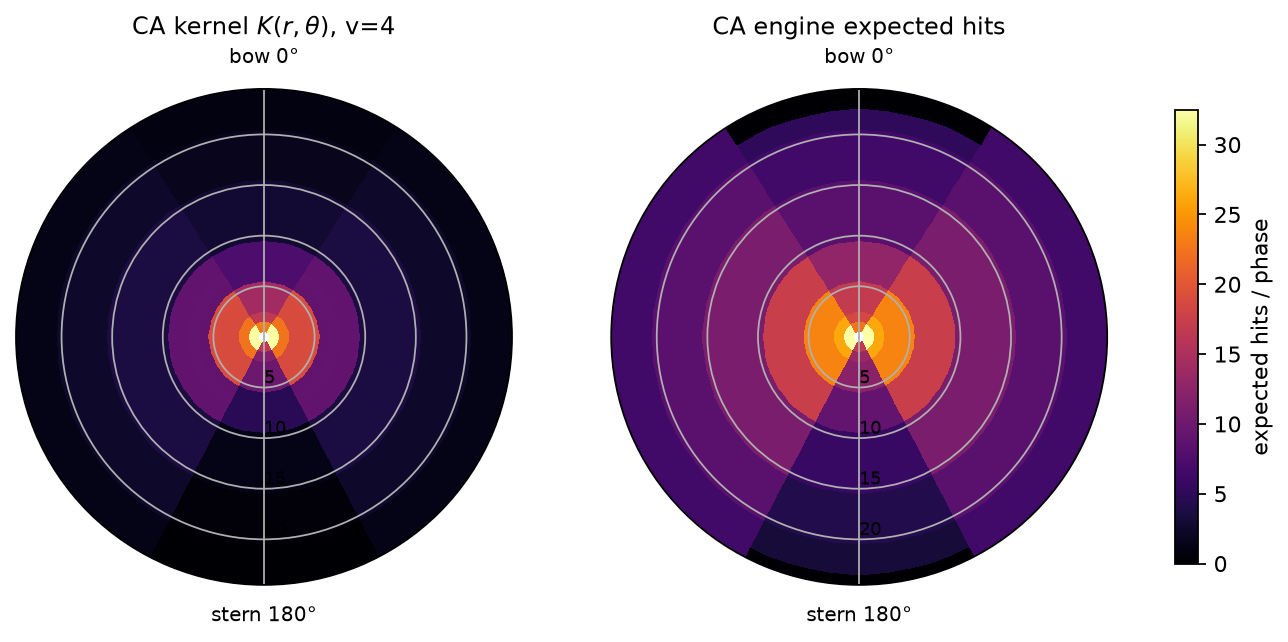
\includegraphics[width=0.85\textwidth]{figures/fig_e01_polar_CA.png}\\[4pt]
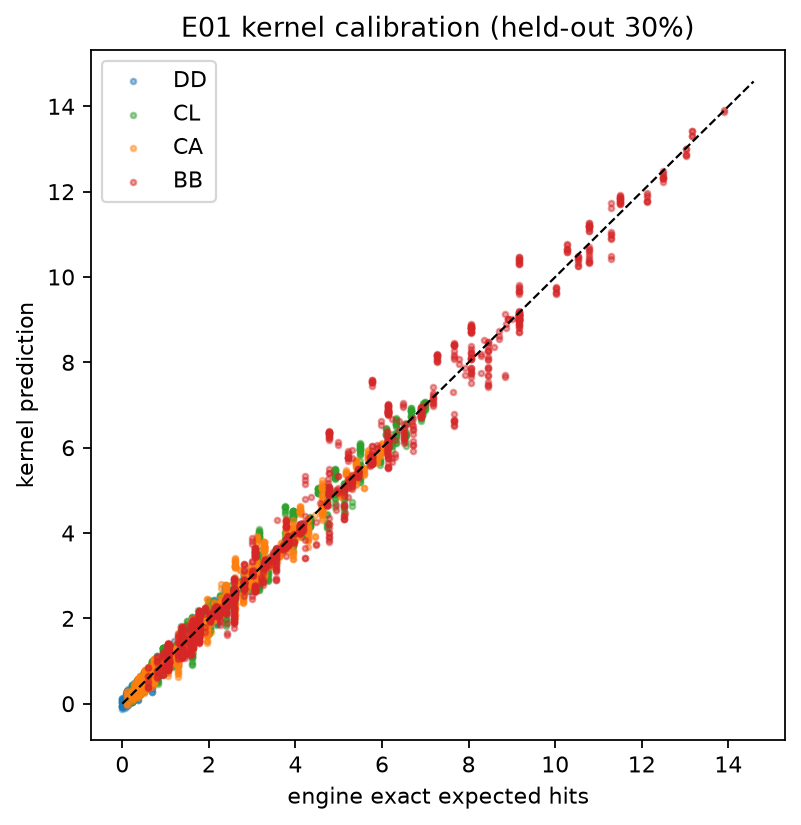
\includegraphics[width=0.6\textwidth]{figures/fig_e01_calibration.png}
\caption{E01 calibration (CA shown as representative; DD/CL/BB maps are
included in the repository results).  Top: heavy-cruister kernel
$K(r,\delta)$ (left) against engine-true expected hits (right) at neutral
target speed; the anisotropy (bow/starboard/stern/port arcs) is structural
and exact.  Bottom: held-out calibration scatter for all four classes.}
\label{fig:kernel}
\end{figure}

\section{Layer 2: The Committed-Maneuver Game (E02)}
\label{sec:game}

\subsection{Reduced state}
Two ships $B,R$ with Dubins-style kinematics reduce by rotational symmetry
to $s=(r,\alpha_B,\alpha_R)$: distance, and the two headings relative to
the line of sight.  The instantaneous payoff is the calibrated
expected-hits differential
\begin{equation}
L(s)=\kB\big(r,\delta_B,v_R,a_R\big)-\lambda\,\kR\big(r,\delta_R,v_B,a_B\big),
\qquad \lambda=1,
\end{equation}
with $\delta_B=-\alpha_B$, $\delta_R=\pi-\alpha_R$, and aspects from the
$\pm30^\circ$ bow/stern sector rule; $\lambda=1$ throughout (asymmetric
value weightings are not explored, and the degeneracy proposition of
Section~\ref{sec:degeneracy} additionally presumes identical kernels).  No
tactical doctrine enters $L$.

\subsection{The degeneracy proposition}\label{sec:degeneracy}
Solving the closed-loop stationary game
$V(s)=\max_{u_B}\min_{u_R}\mathbb{E}[\sum_t\gamma^t L(s_t)]$ by value
iteration on a $(30\times24\times24)$ grid, we observed convergence in two
sweeps with $V\equiv L$ \emph{exactly}.  This is structural:

\begin{proposition}[Symmetric closed-loop degeneracy]\label{prop:deg}
Consider the reduced duel with simultaneous moves, common action set
$U=\{-\omega,0,+\omega\}$ for both players, identical instantaneous
capabilities, and payoff $L$ antisymmetric under the player-swap map
$S(\alpha_B,\alpha_R)=(\alpha_R-\pi,\alpha_B-\pi)$.  If for every state
$s$ the one-step successor-payoff matrix
$X_s[u_B,u_R]=L\big(F(s,u_B,u_R)\big)$ is skew-symmetric in $(u_B,u_R)$,
then the \emph{mixed-strategy} value of every stage game is exactly zero
(von Neumann's minimax theorem), the stationary value equals the
instantaneous differential, $V\equiv L$, and positional maneuvering has
zero equilibrium value.
\end{proposition}
\begin{proof}[Proof sketch]
For a skew-symmetric matrix the uniform strategy of either player caps the
opponent's stage value at $0$, so the stage game's mixed value is $0$ by
the minimax theorem.  Substituting $V=L+\gamma\cdot 0=L$ into the Bellman
operator shows $V\equiv L$ is a fixed point, and $\gamma$-contraction
gives uniqueness.
\end{proof}

Two empirical caveats sharpen the statement.  First, the skew-symmetry
\emph{premise} is satisfied exactly in our formulation: over the entire
grid, $\max|L+L\circ S|=0.0$ for the instantaneous payoff, and the
successor matrices are skew-symmetric to machine precision.  Second, our
value iteration uses \emph{pure}-strategy maximin and still observes
$\max|V-L|=0.0$ (machine precision) at two grid sizes
($16\times12\times12$ and $30\times24\times24$); exact pure saddle
points are stronger than Proposition~\ref{prop:deg} requires; they
appear to reflect the structure of the instant payoff and action set, and
we flag the fully general pure-strategy statement as open.  

  The proposition is the
game-theoretic content of an old practice: maneuvering pays only when
orders are \emph{committed} before the opponent responds---sealed battle
plans---or when capabilities are asymmetric.  It also tells modellers what
NOT to do: a closed-loop PPO/RL agent trained on such a symmetric duel can
at best learn the instantaneous exchange rate.

\subsection{Open-loop (committed) minimax}
Accordingly, E02 solves the \emph{open-loop} game: both sides commit one of
11 sealed heading plans (a turn of $\{0,\pm30,\pm60,\pm90,\pm120,180\}$
degrees executed over three turns---the engine's three-pulse turn
granularity---then hold course), the engagement is simulated under the
calibrated kernels, and the payoff matrix over plan pairs is solved exactly
by linear programming for the mixed-strategy game value.  We scan
$\etav\in\{0.80,0.89,1.00,1.13,1.25,1.33\}$ (speed ratio) $\times$
$\etar\in\{0.75,1.00,1.33\}$ (gun-range ratio, kernel range scaling)
$\times$ three initial geometries (head-on, parallel, crossing),
54 cells in total.

\subsection{Results: tactical regimes and the value of speed}
Figure~\ref{fig:phase} shows the regime maps; Figure~\ref{fig:speed} the
value of speed by geometry.  Three findings:
\begin{enumerate}
\item \textbf{Regimes are stable and interpretable.}  At
$(\etav,\etar)=(1,1)$ the symmetric cells have value $\approx0$ with
pure-strategy saddle points at mutual parallel/oblique courses; away from
symmetry the maximin plan switches between beam-seeking (crossing/parallel
duel), oblique duel, and disengage, with the boundaries reproduced on a
fresh parameter grid ($\etav\in\{0.95,1.05,1.20\}\times
\etar\in\{0.85,1.15\}$) \emph{and} under kernel-calibration
resampling: refitting the kernel on eight bootstrap resamples of the
calibration rows and re-deriving the maximin plans reproduces the plan
identity in $48/48$ cells.
\item \textbf{Role-swap symmetry is exact.}  At the symmetric parameter
cell the game value computed from swapped initial geometries negates to
machine precision ($|V+V_{\text{swap}}|=0.0$), a strong implementation
check.
\item \textbf{Speed's value is geometry-dependent and is not monotone.}
Along $\etav$ at $\etar=1$ (Figure~\ref{fig:speed}) the game value is
$+1.03, +0.84, 0.00, -1.20, -1.39, -1.44$ across
$\etav=0.80\to1.33$ in the head-on geometry, and
$+1.10, +1.10, +0.02, -1.04, -1.49, -1.83$ in the parallel geometry:
under a pure fire-differential payoff with committed plans, the
\emph{faster} side is systematically worse at equal gun range, because
extra speed converts into earlier closure and a longer passage inside the
mutual fire envelope, while it buys no positional term to cash in
(there is no capture objective).  Speed becomes valuable only in
interaction with a range advantage: at $\etar=1.33$ the value is strongly
positive for $\etav\le1$ in the parallel geometry ($+2.8$ to $+3.0$) but
decays through $+0.45$ to $-0.31$ for the fastest ratios, and at
$\etar=0.75$ it is negative throughout ($-0.2$ to $-2.6$); across the
whole scan the range ratio $\etar$ dominates the sign of the value.  The maximin plan identity nevertheless switches at
interpretable speed boundaries with discrete value jumps: in the parallel
geometry the maximin plan is cross/beam-seeking (turn$+60^\circ$) for
$\etav\le0.89$ and oblique duel (turn$-30^\circ$) for $\etav\ge1$,
the switch crossing at $\etav\in(0.89,1.0)$ with a value drop of
$1.08$; in the head-on geometry the disengage regime takes over beyond
$\etav=1.13$.  All boundaries reproduce on the fresh parameter grid.  This is a
substantive refinement of hypothesis H4: in committed duels, speed acts
through the reachable tactical set, and through it alone---without a
positional objective to exploit, speed is worth nothing or less.
\end{enumerate}

\begin{figure}[!htb]
\centering
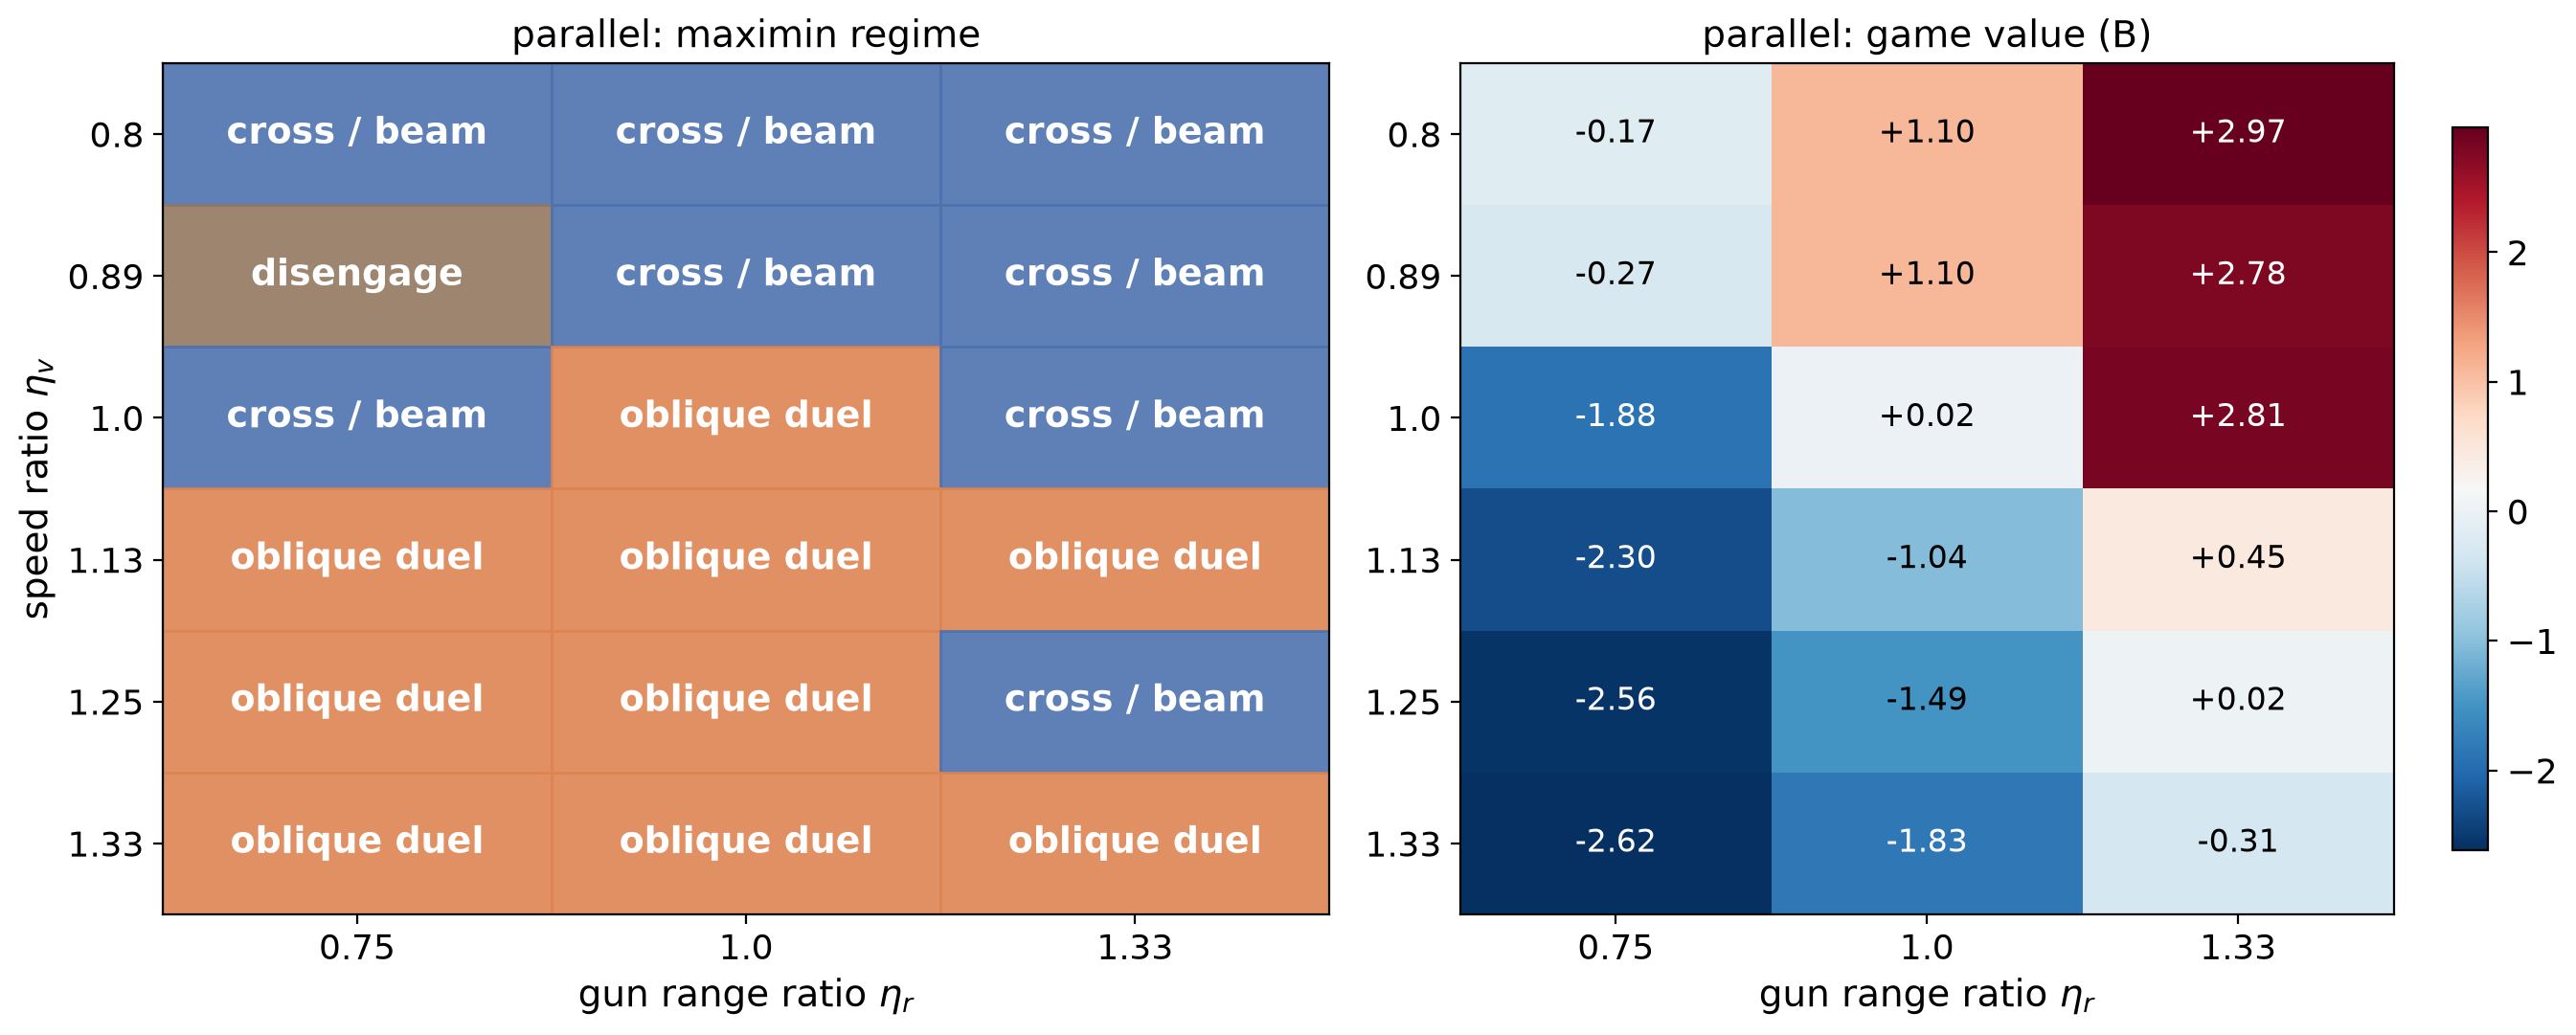
\includegraphics[width=0.98\textwidth]{figures/fig_e02_phase_parallel.png}
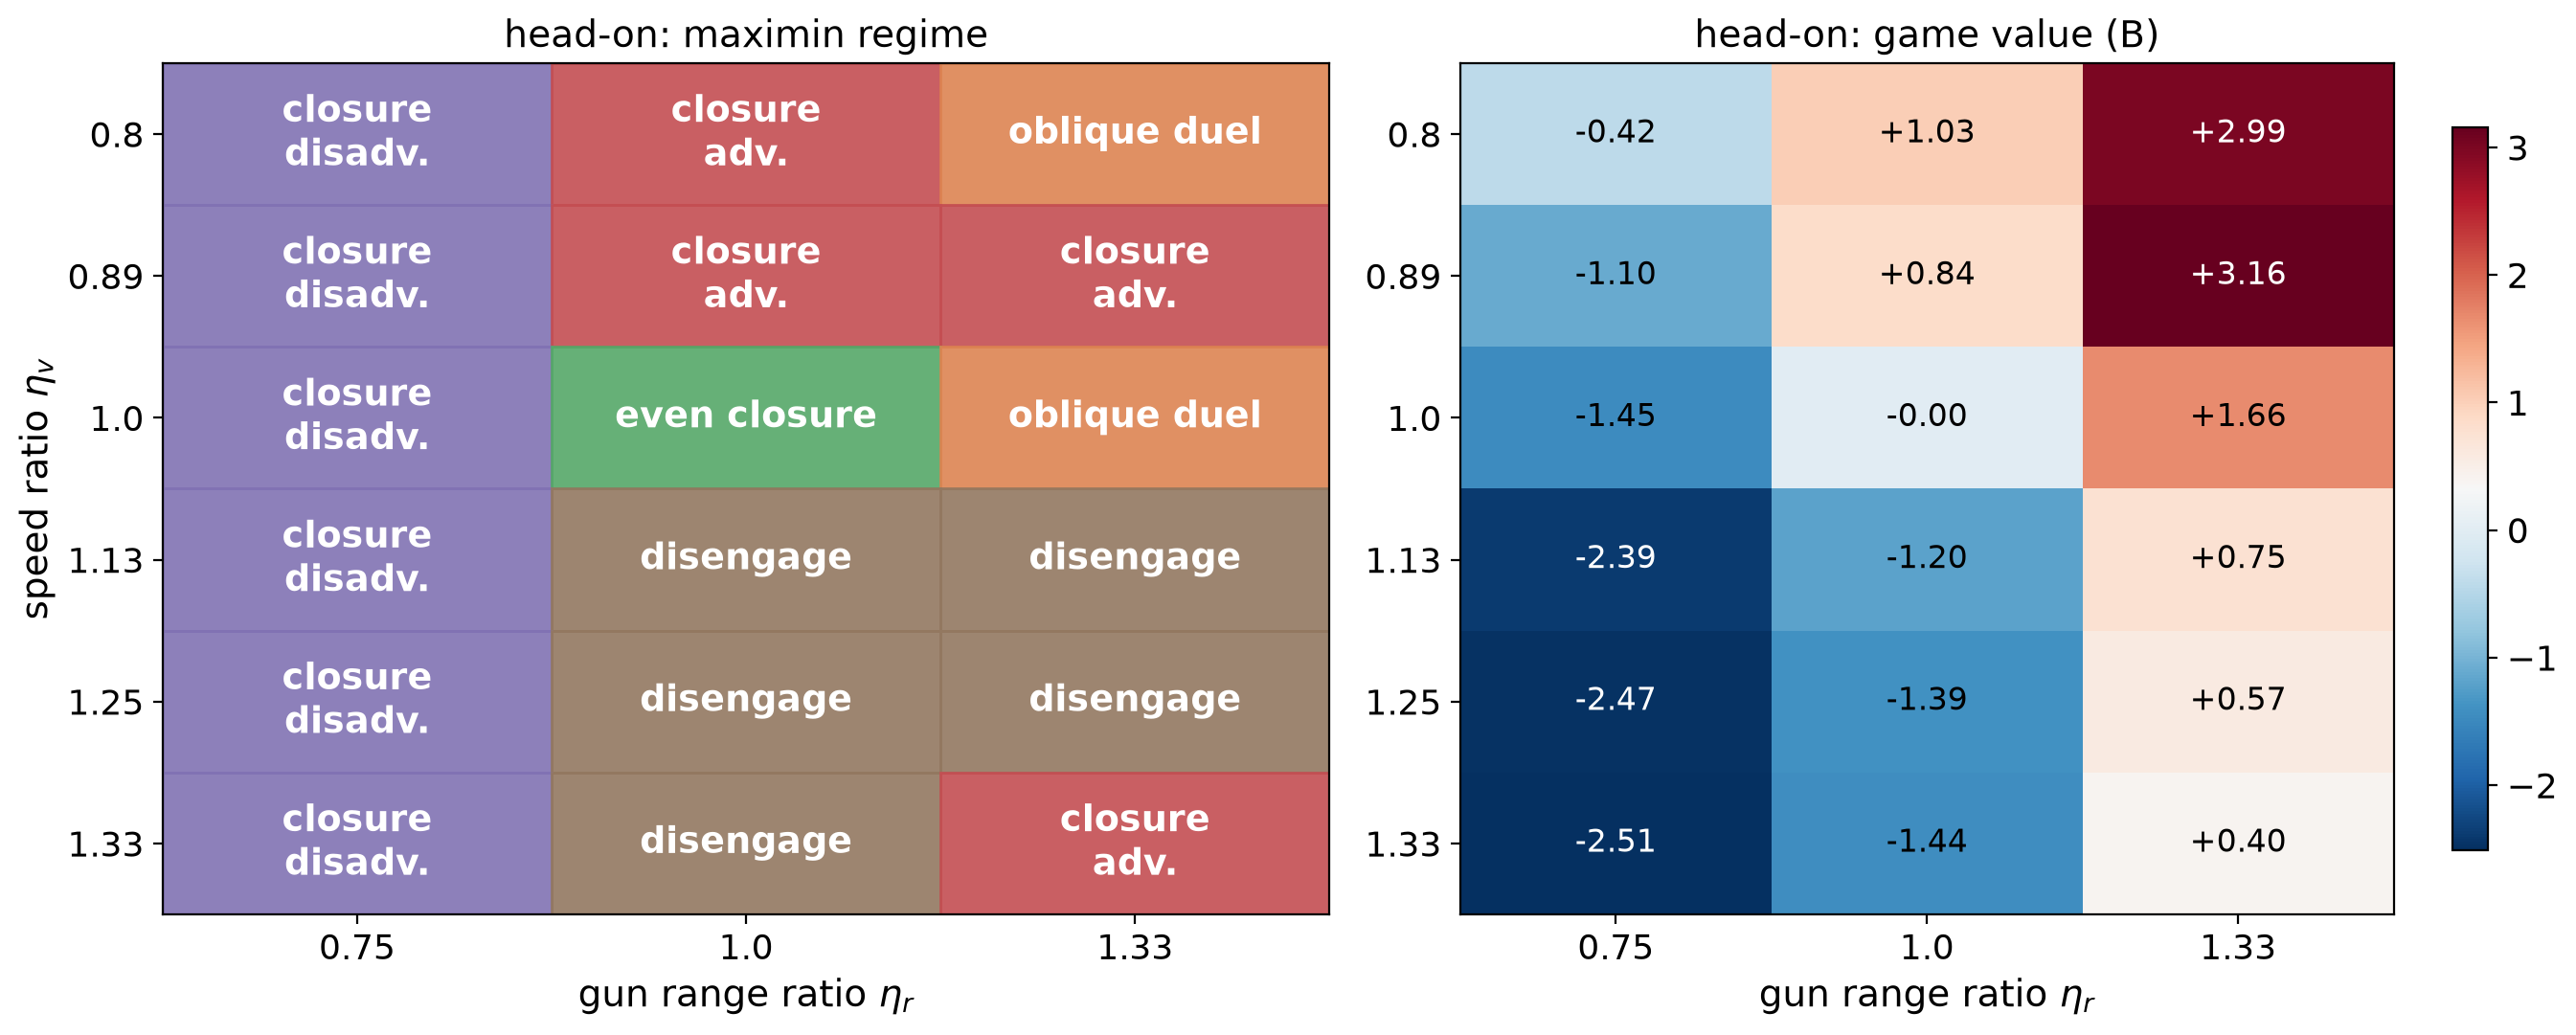
\includegraphics[width=0.98\textwidth]{figures/fig_e02_phase_head_on.png}\\
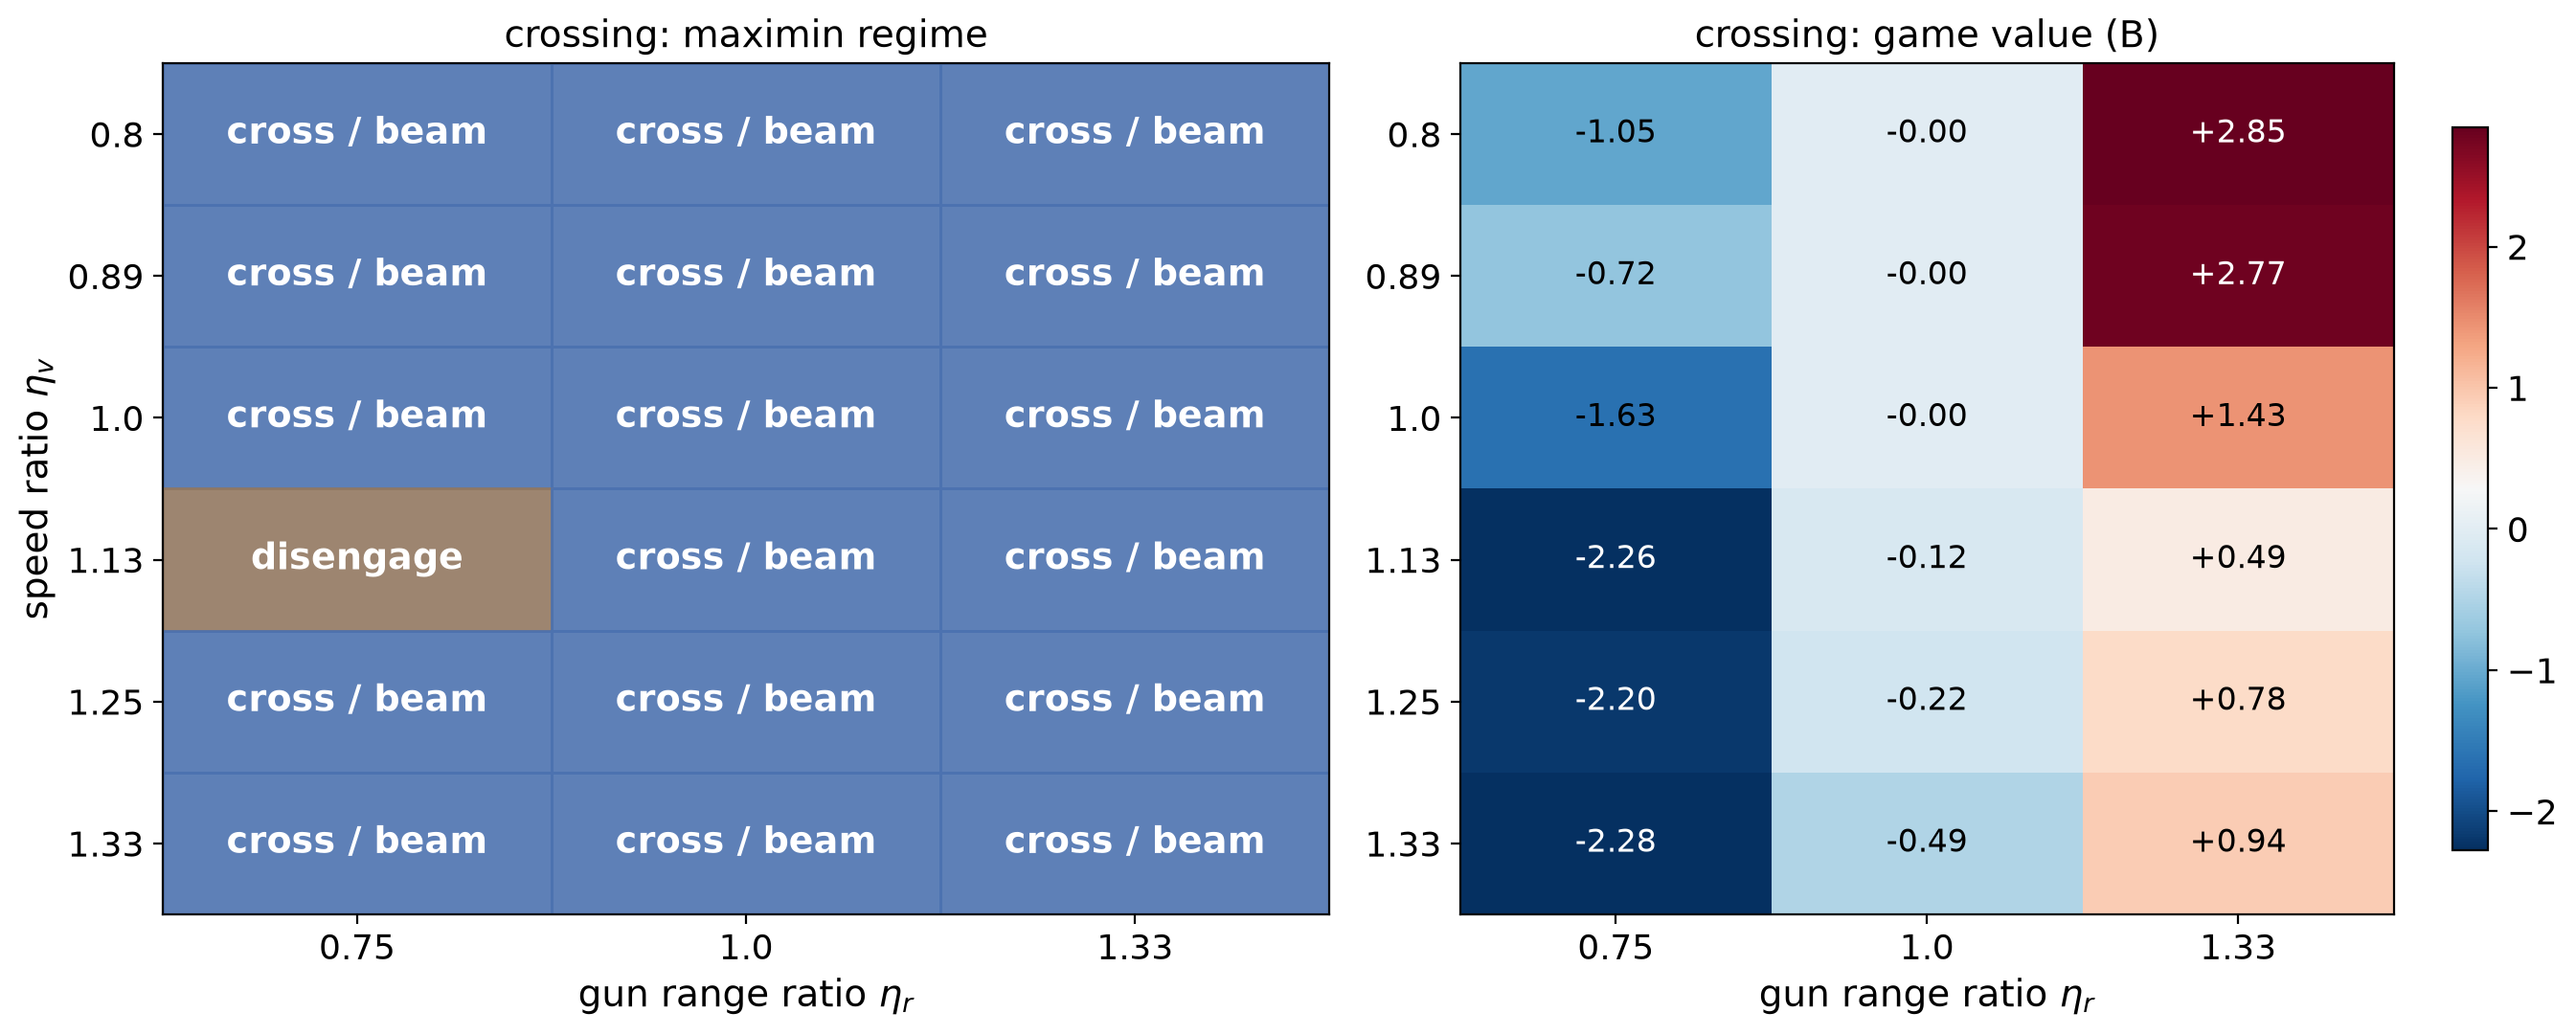
\includegraphics[width=0.98\textwidth]{figures/fig_e02_phase_crossing.png}
\caption{E02 tactical-regime phase diagrams over (speed ratio $\etav$,
gun-range ratio $\etar$) for the three initial geometries.  Left panel of
each pair: dominant regime of the maximin committed plan; right panel:
mixed-strategy game value for B.}
\label{fig:phase}
\end{figure}

\begin{figure}[!htb]
\centering
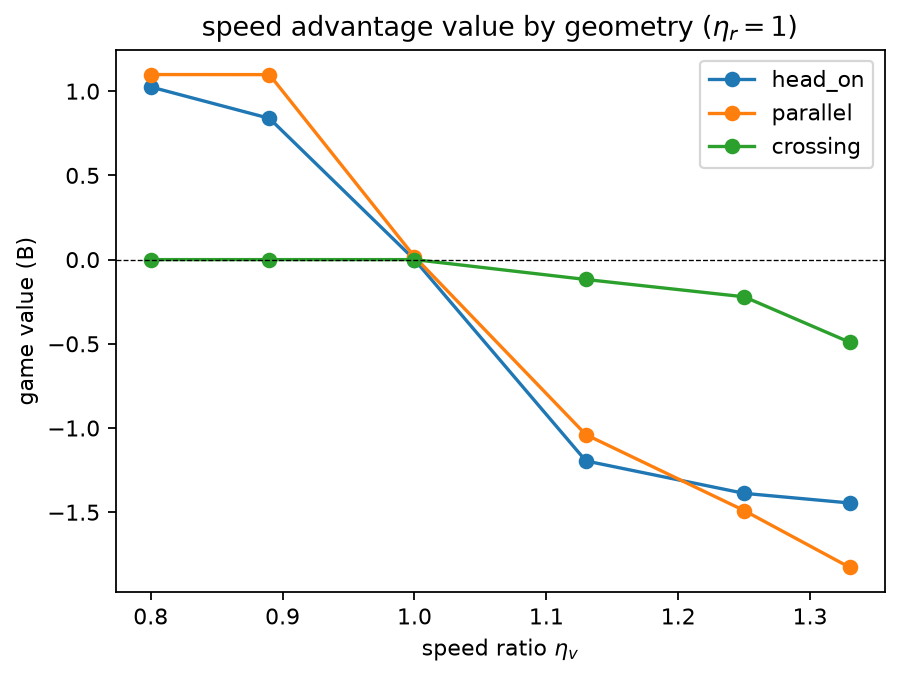
\includegraphics[width=0.6\textwidth]{figures/fig_e02_speed_mechanism.png}
\caption{Speed-mechanism analysis (produced by the E02 script): game value along the speed-ratio axis at
$\etar=1$.  The sign changes are produced by discrete regime switches of
the maximin plan rather than by a continuous exchange-rate shift.}
\label{fig:speed}
\end{figure}

\section{Torpedo Denial (E04)}\label{sec:torpedo}

The plan's central hypothesis (H2) reads $V_{\text{torpedo}} = V_{\text{direct}} + V_{\text{denial}}$, with denial defined strictly by the target's best response: $V_{\text{denial}} = J(\tau_0^*) - J(\tau_T^*)$, where $J$ is the target's gun-position value (\texttt{ship\_gun\_pressure} at hypothetical endpoints, i.e.\ its own expected fire coverage) and $\tau_0^*,\tau_T^*$ are the optimal movement plans without and with the torpedo hazard field.  Critically, the target's decision objective contains only the probabilistic threat---never a damage or doctrine term---so the threat-only regime (plan condition D) is available by construction and the decomposition cannot be manufactured by reward design.

\paragraph{Protocol.}  A destroyer (Fubuki class, Type~90 torpedoes) attacks a
heavy cruiser (Northampton class) across four initial geometries
(chase, opposing, crossing, close) and two force ratios (1v1, 2v1),
36 paired seeds per cell, yielding 216 low-hit plus 72 direct-hit
measurement samples (the direct-hit pool exists only in the close
geometry).  Both sides sail fixed
straight plans for one turn through the engine's formal
submit/advance pipeline (zero dice: A/C/D conditions share byte-identical
states); at the torpedo-planning phase the attacker's full legal launch
space (launcher $\times$ side $\times$ angle $\times$ speed setting $\times$
launch impulse, each validated by \texttt{validate\_orders}) is enumerated,
each track is projected by the engine's own impulse-loop model (verified
cell-by-cell against a real adjudicated launch), and the cruiser's best
response is recomputed over its complete legal plan space
(340--600 plans) with and without the hazard.  All denial values are in units of the gun-position value $J$; normalized values divide by the reference position value $J_{\text{ref}}=J(\tau_0^*)$.  The threat weight $w=0.343$
is the engine collision table's expected damage fraction for the cruiser's
displacement band (36-outcome enumeration); $w=1$ (the plan's raw form) is
reported as a sensitivity.

\paragraph{Results.}  In the \emph{low-direct-hit} subset
($\mathbb{E}[\text{hits}] = 0.083$; $n=216$), $V_{\text{denial}}$ is
structurally identical to zero---all 216 samples equal $0$ exactly (the
bootstrap interval degenerates to $[0,0]$)---in \emph{every} geometry and
under all threat weightings ($w=0.343$, $w=1$, and constant-threat
condition D).  The pre-specified acceptance (denial above zero in at least
three geometries) therefore \textbf{fails}, and we report it as a null
result with its mechanism.  The mechanism is quantitative and, we argue,
general: the engine's coarse hit-table granularity makes the target's
gun-position value landscape \emph{tiered}: each measurement's plan space
holds 340--600 legal plans, within which $J$ takes on average only 8
distinct values (4--14 across cells), and the top tier
($J/J_{\text{ref}}=1$) is shared by 25.5 tied routes on average
(12--32.5 across cells).  A single torpedo track is a thin
line in $(\text{hex},\text{impulse})$ space: it can intersect some members
of the top tier, but never the whole tier, so the target re-optimizes to a
tied route at zero value loss (route change is real---$100\%$ of samples
change course, by $1.67\times60^{\circ}$ on average---but $J$ is preserved).
The threat's discounted expected cost under the top tier
($w\cdot P_{\text{hit}} \approx 0.343\times0.083 \approx 0.029$) is an order
of magnitude below the tier gap ($0.58$), so the conclusion is invariant to
the threat weighting.

In the \emph{direct-hit} control ($\mathbb{E}[\text{hits}]\in[0.42,1.14]$;
$n=72$), the track lies directly on the top-tier cluster and denial value
appears: $V_{\text{denial}} = 0.92$ hull-value points ($95\%$ CI $[0.42, 1.42]$;
normalized $0.0264$), while route\emph{changing} becomes rare ($15.3\%$)---with
the whole cluster priced out, no tied refuge exists.  The decomposition
$V_{\text{torpedo}} = V_{\text{direct}} + V_{\text{denial}}$ itself is
confirmed: both components are measurable, disjoint, and the low-hit
torpedo value is pure direct value ($V_{\text{torpedo}} = 0.0285 =
V_{\text{direct}} + 0$).

\begin{figure}[!htb]
\centering
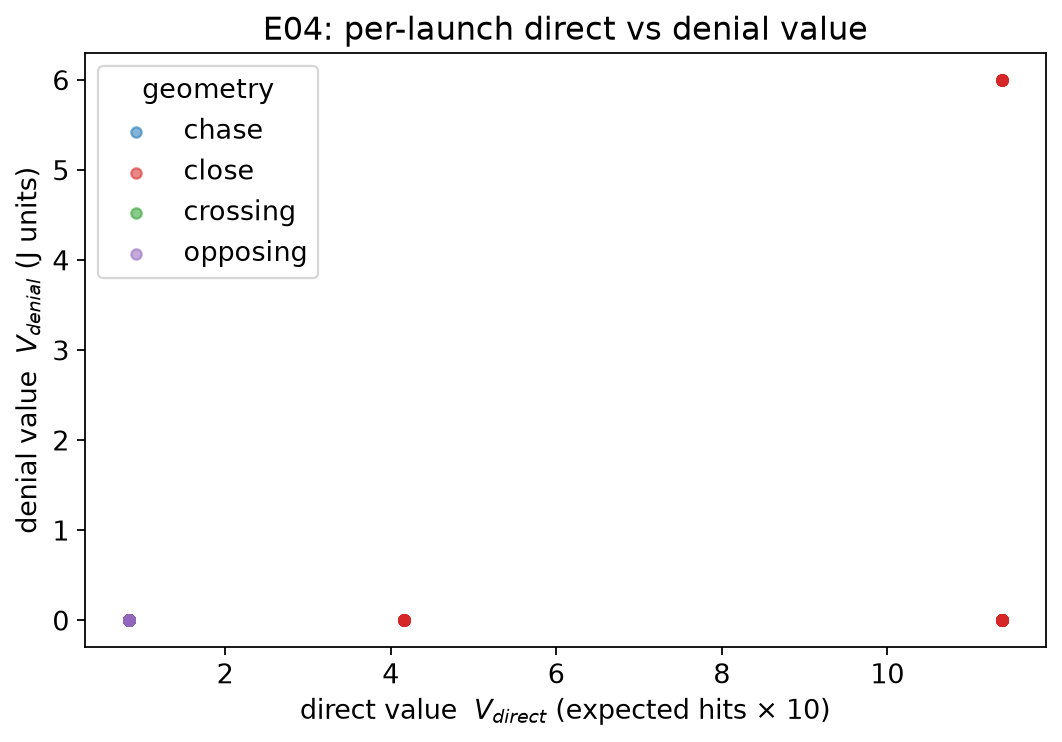
\includegraphics[width=0.62\textwidth]{figures/fig_e04_decomposition.png}
\caption{E04.  Direct value versus denial value of individual launches
by geometry (direct value plotted in expected-hits $\times 10$ units):
denial concentrates in the direct-hit (close) geometry, while
low-direct-hit launches (near zero on the $x$-axis) yield none.}
\label{fig:e04}
\end{figure}

\paragraph{Deviations from the pre-analysis plan and design confounds.}
Two protocol deviations occurred before measurement and are recorded in
the repository's experiment log: (i)\ the originally planned
``launch on turn~1, response on turn~2'' design proved structurally
infeasible---a pilot scan of $\approx700$ candidate geometries showed the
turn-1 track already sweeps the target's turn-2 reachable set, collapsing
every contact into close broadside shots---so the protocol measures
same-turn perfect-information responses, mirroring the engine's own
torpedo-assist intercept model; (ii)\ geometries were selected by the
same pilot scan so that a stable low-hit opportunity pool exists.  The
analysis gates were fixed in the project's planning document and scripts
before the measurements reported here; no external registry was used.
Two design confounds qualify the direct-hit contrast: it comes from a
single geometry (close), jointly changing range, hit expectancy, and
track-tier overlap; and the low-hit pool's $\mathbb{E}[\text{hits}]$ is
constant at $1/12$ (zero variance), so the ``low-hit regime'' is a single
point of the hit distribution.  A geometry $\times$ salvo-size factorial
that separates these factors is the natural continuation.

\begin{figure}[!htb]
\centering
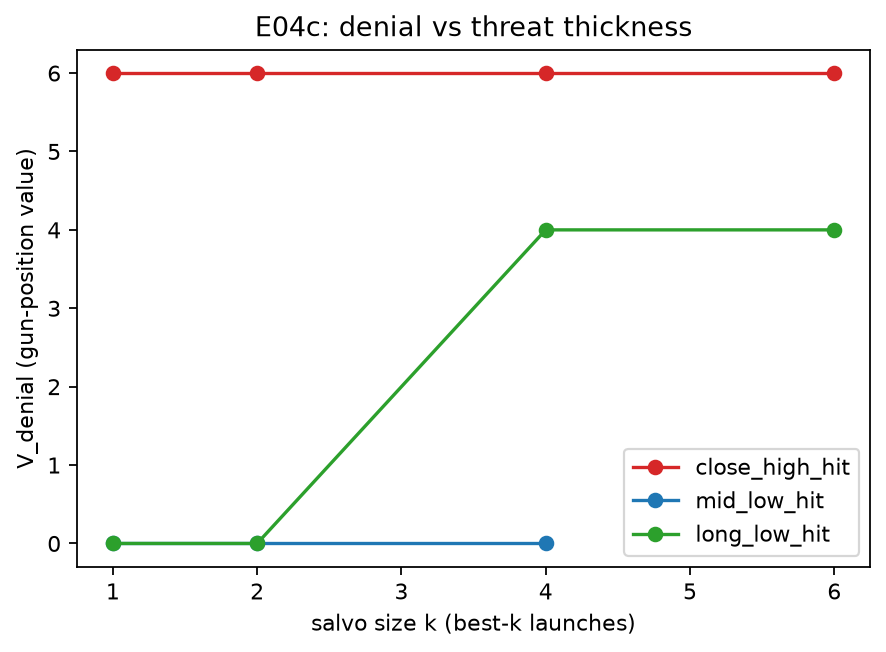
\includegraphics[width=0.6\textwidth]{figures/fig_e04salvo_curve.png}
\caption{E04c: denial value versus salvo size $k$ by geometry
(deduplicated sweep).  Denial is flat to $k{=}4$ and rises at $k{=}6$
where the route-change rate reaches $100\%$; the low-hit stratum shows
no denial at $k\le2$, $+2.0$ at $k{=}4$, and $+4.0$ at $k{=}6$.}
\label{fig:e04c}
\end{figure}

\paragraph{Salvo-size sweep (E04c).}  Denial as a function of threat
thickness identifies the mechanism directly.  Sorting the attacker's
launches by expected hits and combining the top-$k$ tracks
($k=1,2,4,6$; $30$ paired seeds per geometry, $270$ deduplicated
measurements, decision-level protocol): the direct value grows linearly
with $k$ (mean $2.6\to5.1\to10.2\to20.2$ target-value points), while
denial rises monotonically but convexly ($2.0\to2.0\to3.3\to5.0$) and
the route-change rate reaches $100\%$ only at $k=6$.  In the low-hit
stratum the denial value is monotone in thickness: $0$ at $k\le2$
($n=60$), $+2.0$ at $k=4$ ($n=60$), and $+4.0$ at $k=6$ ($n=30$).  Even the refined H2
statement---``thin low-hit threats have no denial value; thickness is
what buys it''---is thus directly visible in the data, with the caveat
that the exact threshold depends on the threat-weighting normalization.

\paragraph{Interpretation.}  ``Torpedoes that miss but change the battle''
do happen in this engine---as course changes that preserve gun value.  The
maneuver-denial value of a thin low-probability threat is exactly zero
against a tiered value landscape with tied alternatives; denial value is
realized only when the threat saturates the target's entire top position
tier (massed salvoes at close range, or the constant-threat perception
regime D, where the same tracks yield $V_{\text{denial}}^{(D)}=0.2126$).
This refines H2 into a testable structural claim: denial value is governed
by the interaction between threat thickness and the tie structure of the
position-value landscape, not by hit probability alone.

\section{Engine-in-the-Loop Validation (E06)}\label{sec:validation}

The continuous policy is translated into legal engine orders by a
\emph{geometry policy}: at each movement-planning phase it measures the
true geometry, re-solves the committed-maneuver game (receding horizon,
three-turn commitment), and selects among the engine's own legal movement
candidates the plan best matching the maximin heading change at preserved
speed; gunnery targets maximize expected hits $\times$ target value.
Translation is audited by the engine's order validator; no engine state is
mutated and no hidden information is read.

We validate on a near-symmetric cruiser duel (San Francisco class vs.\
New Orleans class) under three initial geometries, 60 paired seeds per
cell.  The ALLIES side is always the mature \emph{balanced} doctrine
commander; the three compared policies all play the AXIS side (so
``vs.\ line'' and ``vs.\ straight'' below are alternative AXIS policies,
each still facing the same \emph{balanced} opponent).  Against the non-maneuvering \emph{straight} baseline
the geometry policy produces a large, significant paired damage
differential in every geometry: $+7.7$ [$+6.4,+9.0$] in the parallel
geometry ($93\%$ of pairs positive), $+9.6$ [$+8.1,+11.0$] in the
crossing geometry ($93\%$), and $+5.2$ [$+3.6,+6.8$] head-on ($78\%$).
Against the doctrine profiles the picture is differentiated and honest:
the only doctrine cell whose $95\%$ interval excludes zero
(uncorrected; one of nine comparisons) is \emph{head-on vs.\ line},
where the line-ahead specialist \emph{beats} the geometry policy
($-1.73$ [$-3.23,-0.28$]); everywhere else the policy is at parity with
the doctrine commanders (all remaining CIs include zero; the crossing cell
against \emph{balanced}, $+1.47$ [$-0.03,+3.02$], is borderline).  The
degeneracy proposition predicted exactly this shape of result: in a
symmetric duel a mature heuristic already captures most positional
value, so the surrogate's contribution is to \emph{guarantee} competent
geometry from first principles---and to concede, gracefully, where a
tuned specialist doctrine has an edge.  Figure~\ref{fig:e06} shows the
paired forest plot.

\begin{figure}[!htb]
\centering
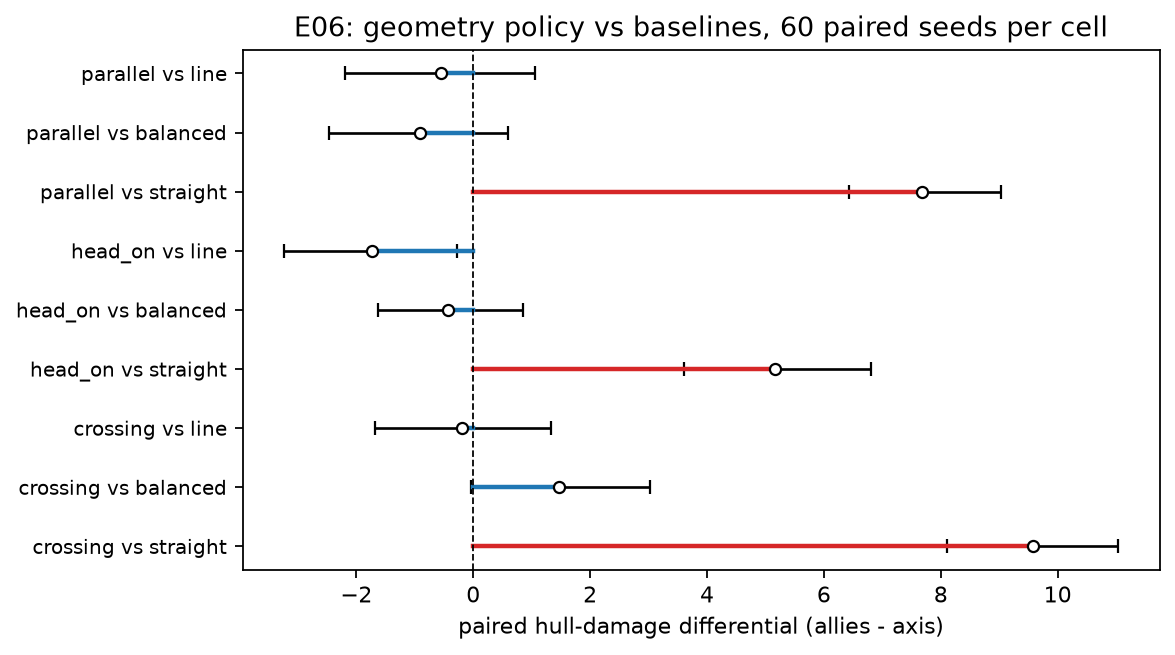
\includegraphics[width=0.8\textwidth]{figures/fig_e06_forest.png}
\caption{E06 paired validation.  Mean paired hull-damage differential
(allies minus axis; positive favors the geometry policy) with bootstrap
$95\%$ CIs, 60 paired seeds per cell.}
\label{fig:e06}
\end{figure}

\paragraph{Historical external-validity check (E07).}  As a qualitative
check outside synthetic geometries, the same translation layer plays the
Japanese side of the historical Cape Esperance scenario (IBS-S-01, with
its historical special rules active: allied fire halved, axis no-fire
first turn, allied reinforcements), 20 seeds attempted per policy; three runs per
policy were dropped after reinforcement-phase exceptions (unevenly across
policies, so selection bias cannot be excluded), leaving 17/15/20 usable
paired games.  The
pattern matches and sharpens the synthetic validation: the geometry
policy out-damages the straight baseline by $+12.2$ hull points ($95\%$
CI $[+6.5,+17.9]$, $86\%$ of pairs positive) and runs ahead of the
\emph{line} doctrine by $+3.7$ ($[-2.4,+9.6]$)---a positive trend that
does not reach significance.  The axis side loses on
all policies (win rate $0\%$), consistent with the scenario's known
allied bias in the engine's own benchmark (484 allied vs.\ 174 axis
decisive outcomes; \texttt{benchmarks/ibs-s01-r30/README.md}), so no
tactical claim is drawn from the win column.

\section{Geometry-Induced Engagement Networks: A Specification
Analysis (E05)}\label{sec:engagement}

The plan hypothesizes (H3) that geometry-induced network features (local
force ratio, attacker concentration, formation algebraic connectivity)
predict next-phase damage beyond aggregate fire totals, with acceptance
$\Delta R^2\ge+0.05$ or MAE improvement $\ge10\%$.  We ran 120 games
(600 turn snapshots; 5{,}862 ship-turn samples; damage windows cross-checked
against event payloads, 2{,}535/2{,}535 hull points), built directed
graphs with engine-true expected-fire edge weights under night-visibility
gating, and compared OLS models on an 80/20 game-level split.

Result: adding graph features yields $\Delta R^2=+0.0330$ ($95\%$ CI
$[+0.0069,+0.0561]$) and a logistic-detection AUC gain of $+0.0286$
($[+0.0119,+0.0459]$), but a slightly \emph{worse} MAE ($-0.011$
$[-0.037,+0.015]$).  The specification, however, is decisive, and the
plan's own metric list resolves it: \S6.2 of the plan defines the graph
metrics to include the \emph{weighted in-degree} ($P_B(j)$, the incoming
directional expected fire)---so under the plan-literal reading the
baseline may contain only non-graph totals (hull fraction, speed, mean
enemy distance, force ratio) and every directed-fire quantity belongs to
the graph set.  Re-estimating under this plan-literal specification with the
reproducible script \texttt{e05\_spec\_analysis.py} (game-level
bootstrap, 500 resamples; point estimates stored), the engagement graph
passes both gates: $\Delta R^2 = +0.108$ ($95\%$ CI $[+0.069,+0.160]$)
and a relative MAE reduction of $17.5\%$ ($95\%$ CI
$[9.7\%,26.7\%]$).  The
honest summary: \emph{the directional in-degree is the graph}.  Once it
is admitted as a network quantity---as the plan's metric list
instructs---geometry-induced engagement networks carry substantial
predictive value beyond aggregate force ratios, while the pure
\emph{shape} refinements (local force ratio, concentration, algebraic
connectivity) add little beyond it; under the stricter reading, where
even the in-degree is a baseline covariate, only the shape features
remain and they add $+0.033$ ($[+0.007,+0.056]$), below the gate, with a
slightly worse MAE.  Both specifications, point estimates, and both
bootstrap protocols (sample-level and game-level) are reported in the
repository so the reader can take either reading.  Out-of-sample
transfer across scenarios is negative (train S-01, test S-03 and vice
versa), bounding the claim to within-scenario prediction.

\begin{figure}[!htb]
\centering
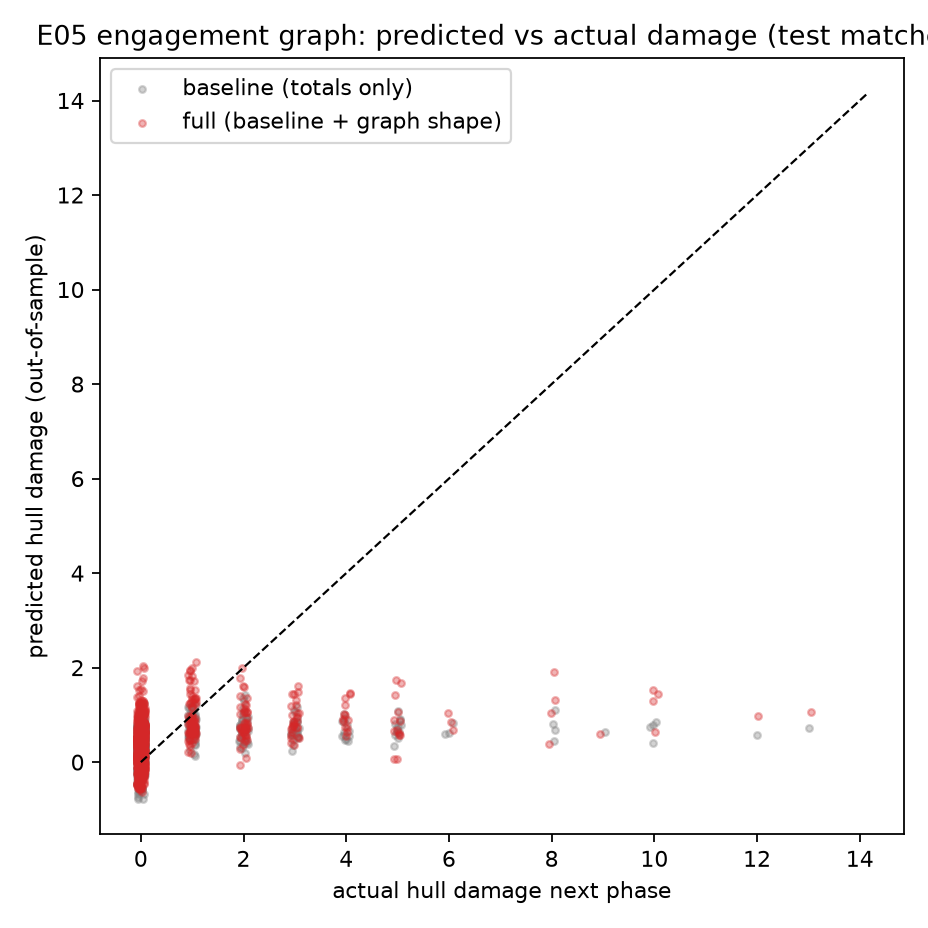
\includegraphics[width=0.49\textwidth]{figures/fig_e05_scatter.png}
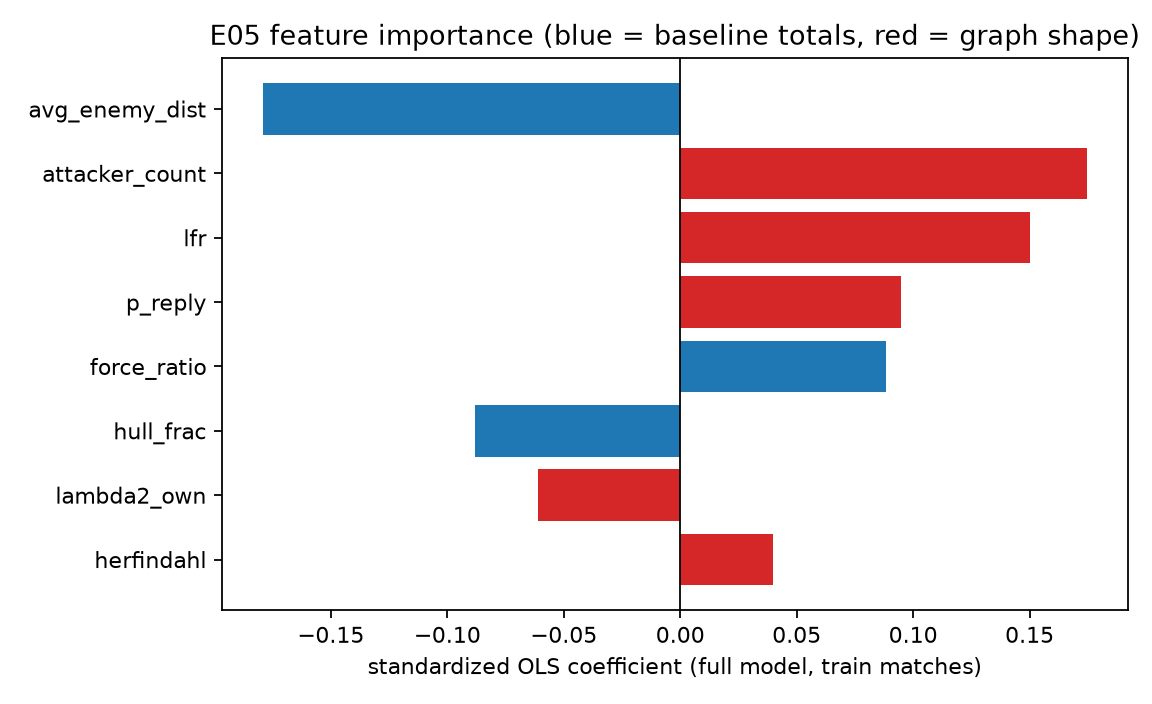
\includegraphics[width=0.49\textwidth]{figures/fig_e05_feature_importance.png}
\caption{E05.  Left: predicted vs.\ actual next-phase hull damage
(model with graph features).  Right: standardized OLS coefficients
(blue = baseline totals, red = graph-shape features).}
\label{fig:e05}
\end{figure}

\section{Discussion}\label{sec:discussion}

\paragraph{Why doctrine exists.}  The degeneracy proposition gives a
compact answer to ``why is crossing the~T a doctrine rather than an
equilibrium strategy?'': in the closed loop, against a free and informed
opponent, positional play is worthless; it becomes valuable exactly when
plans are committed (as in real naval combat and in the engine's sealed
orders), when capabilities are asymmetric (speed, range, firepower), or
when information is incomplete.  The open-loop analysis then localizes
\emph{where} the classical maneuvers are optimal (Figure~\ref{fig:phase}).

\paragraph{What the kernel buys.}  A smooth, direction-resolving surrogate
with $\rho\approx0.99$ makes continuous admissible the machinery of
differential games against a complete discrete ruleset, and the inversion
+ censored-regression calibration is generic: any table-driven engine can
be surrogated the same way.

\paragraph{Limitations.}  (i)~The surrogate is calibrated per ship
class-pair on open-water geometry; terrain, smoke, radar illumination and
formation effects are not in $L$.  The isotropic-kernel control and the
six cross-pair transfers of E01b bound what the calibration certifies,
but an axial-walk-bearing baseline and further unseen pairs remain
future work.  (ii)~The plan library is coarse;
finer adaptive plan families would sharpen regime boundaries.
(iii)~Constant-cruise approximation omits speed-throttle tactics (torpedo
evasion by slowdown is E04's province and is modeled through the hazard
field instead).  (iv)~The historical scenarios partially execute their
special rules (per the engine's coverage ledger); we therefore validate on
synthetic symmetric engagements rather than claimed historical replays.
(v)~In the phase diagram, the small positive values of the \emph{slower}
side at equal range (e.g., $+1.1$ at $\etav=0.8, \etar=1$) are counter-intuitive; they arise from the mixed-strategy value over the committed-plan matrix once the pass-through kinematics of the surrogate (no
collision, range clamped at half a hex) break exchange symmetry, and we
flag them as model artefacts pending a collision-aware treatment rather
than as tactical claims.
(vi)~The engine is a wargame, not physics: conclusions are about the rules
system, with historical doctrines as qualitative external anchors.

\section{Reproducibility}\label{sec:repro}
\begin{table}[t]
\centering\small
\caption{Pre-specified acceptance summary.  The E04 low-hit gate fails
and is reported as an honest null with its mechanism
(Section~\ref{sec:torpedo}); the E05 gate is specification-sensitive and
both readings are reported (Section~\ref{sec:engagement}); nothing was
tuned post hoc.}
\label{tab:acceptance}
\begin{tabular}{p{2.6cm}p{4.6cm}p{6.2cm}}
\toprule
Experiment & Gate & Outcome \\
\midrule
E00 audit & zero leakage / zero mutation / determinism & PASS \\
E01 kernel & $\rho\ge0.90$, nMAE $\le0.15$ & PASS ($\rho=0.991$, $0.057$) \\
E02 game & regime stability, swap symmetry & PASS (swap $0.0$; $48/48$ resample stability) \\
E04 torpedo & denial CI $>0$ in $\ge3$ low-hit geometries & FAIL ($\equiv 0$; tiered-value mechanism) \\
E05 network & $\Delta R^2\ge+0.05$ or MAE $-10\%$ & PASS (plan-literal: $\Delta R^2=+0.108$); strict: $+0.033$ \\
E06 validation & translated policy competitive & PASS ($\gg$ straight; parity except head-on vs.\ line) \\
\bottomrule
\end{tabular}
\end{table}

\sloppypar{Every experiment is a script under \texttt{research/experiments/}
(\texttt{e00\_engine\_audit}, \texttt{e01\_fire\_kernel},
\texttt{e01b\_kernel\_baselines}, \texttt{e02\_crossing\_t\_phase},
\texttt{e04\_torpedo\_denial}, \texttt{e04c\_salvo\_sweep},
\texttt{e05\_engagement\_graph}, \texttt{e06\_engine\_validation},
\texttt{e07\_historical\_check}) writing
raw CSV/JSON plus figures under \texttt{research/results/}.  All runs are
seeded; paired comparisons share scenario, seed and initial placement;
confidence intervals are bootstrap or exact (matrix-game LP).  The frozen
engine commit for every number in this paper is \texttt{fc77a65}
(\url{github.com/fuxiaoji/iron-bottom-sound}).  The engine
commit, rule-coverage ledger, and the research-layer discipline (no
adjudication modification, no hidden-information use, no tactical terms in
objectives) are audited by E00.}

\section{Conclusion}
Directional firepower, committed maneuver, and torpedo threat can be
studied as one measurable system when a complete, deterministic wargame
engine serves as the calibration and validation substrate.  The calibrated
kernel reaches $\rho=0.99$ fidelity; the degeneracy proposition explains
why naval tactics are commitments and what RL on symmetric duels can and
cannot learn; the committed-maneuver game maps tactical regimes across
speed and range asymmetries; the translated geometry policy survives
engine validation against doctrine baselines; the engagement-network
analysis passes its gates under the plan's own metric definitions, with
its specification boundary mapped; and the torpedo-denial null locates
exactly where doctrine intuition outruns the rules structure.  We view the
pipeline---engine, kernel, committed-maneuver game, translation layer,
audit---as the durable contribution.

\appendix
\section{Fitted Range Modifiers vs.\ the Engine's Bands}
\label{app:modifiers}
Table~\ref{tab:appendix-modifiers} compares, for every attacker class,
the kernel's fitted range-modifier curve $M_r$ (evaluated at the engine's
seven band centers) with the engine's discrete band values.  The residual
$\approx$+1.2-point offset is common to all four classes (5.17--5.24 at
the long-range band), consistent with an absorbed constant modifier
rather than a per-class effect; the ship-to-ship consistency of the
fitted curves (e.g., band 1: $-24.8$ to $-24.9$ across all four classes)
is the calibration's self-check.

\begin{table}[h]
\centering\small
\caption{Fitted $M_r$ at the engine's band centers (primary battery,
neutral target speed, broadside aspect) against the engine's discrete
band values.}
\label{tab:appendix-modifiers}
\begin{tabular}{lccccccc}
\toprule
Band center (hex) & 1 & 2 & 4 & 7.5 & 12.5 & 18 & 22+ \\
Engine band value & $-24$ & $-15$ & $-12$ & $-6$ & $0$ & $+2$ & $+4$ \\
\midrule
DD (Laffey) & $-24.9$ & $-16.4$ & $-13.3$ & $-4.8$ & $+1.3$ & $+3.2$ & $+5.2$ \\
CL (Helena) & $-24.8$ & $-16.5$ & $-13.4$ & $-4.8$ & $+1.2$ & $+3.2$ & $+5.2$ \\
CA (San Francisco) & $-24.9$ & $-16.4$ & $-13.4$ & $-4.8$ & $+1.2$ & $+3.2$ & $+5.2$ \\
BB (Yamato) & $-24.8$ & $-16.5$ & $-13.4$ & $-4.8$ & $+1.2$ & $+3.2$ & $+5.2$ \\
\bottomrule
\end{tabular}
\end{table}

\section{Per-Class Kernel Maps (DD, CL, BB)}
\label{app:polars}
Figure~\ref{fig:app-polars} completes Figure~\ref{fig:kernel} with the
calibrated kernel maps of the remaining attacker classes (CA shown in the
main text).  The class signature is visible in the anisotropy: the
destroyer's map is confined to short range with a near-symmetric
four-lobe pattern, the light cruiser shows the classic broadside
butterfly, and the battleship combines long range with a heavy
stern-sector deficit.

\begin{figure}[h]
\centering
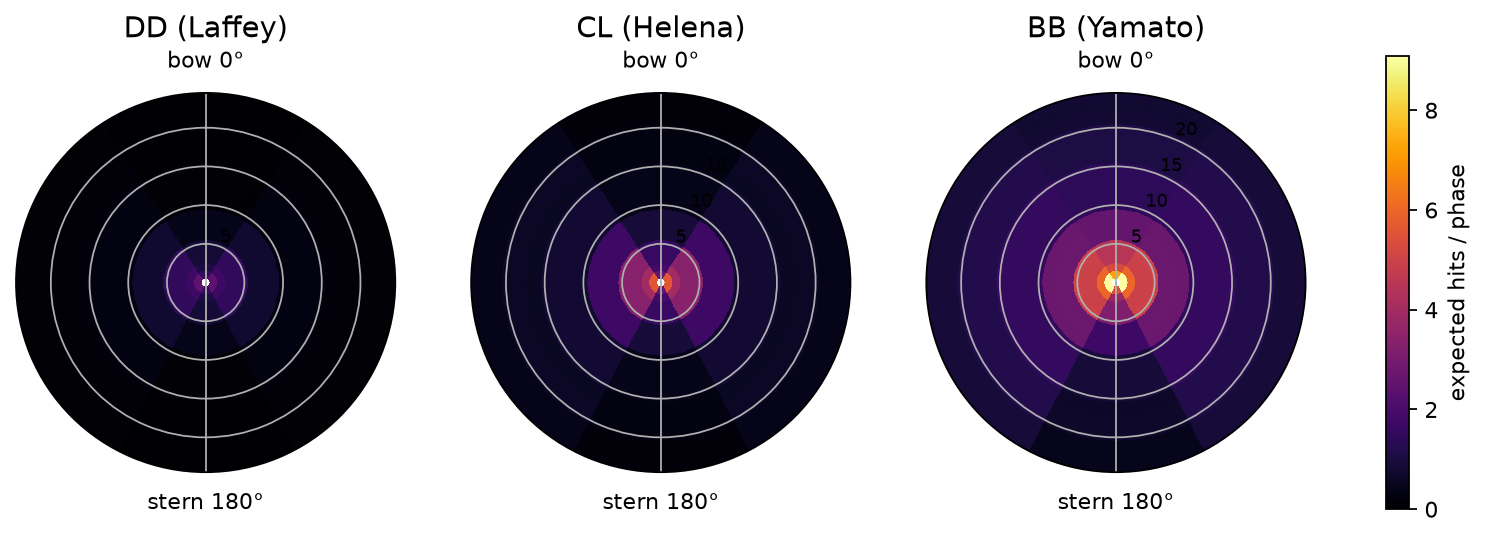
\includegraphics[width=0.85\textwidth]{figures/fig_e01_polars_appendix.png}
\caption{Per-class calibrated kernel maps $K(r,\theta)$ at neutral
target speed.  Left: destroyer (Laffey).  Center: light cruiser (Helena).
Right: battleship (Yamato).}
\label{fig:app-polars}
\end{figure}

\bibliographystyle{unsrtnat}
\begin{thebibliography}{20}

\bibitem{bernotti1911}
R.~Bernotti, ``The fundamentals of naval tactics,'' \emph{U.S. Naval
Institute Proceedings}, vol.~37, 1911.

\bibitem{bernotti1912}
R.~Bernotti, ``The fundamentals of naval tactics (continued),'' \emph{U.S.
Naval Institute Proceedings}, vol.~38, 1912.

\bibitem{taylor1974}
J.~G. Taylor, ``Lanchester-type models of warfare and optimal control,''
\emph{Naval Research Logistics Quarterly}, vol.~21, no.~1, pp.~79--106,
1974.

\bibitem{protopopescu1989}
V.~Protopopescu, R.~T. Santoro, and J.~Dockery, ``Combat modeling with
partial differential equations,'' \emph{European Journal of Operational
Research}, vol.~38, no.~2, pp.~178--183, 1989.

\bibitem{gonzalez2011}
E.~Gonz{\'a}lez and M.~Villena, ``Spatial Lanchester models,'' \emph{European
Journal of Operational Research}, vol.~210, no.~3, pp.~706--715, 2011.

\bibitem{networked2020}
A.~C. Kalloniatis, K.~Hoek, M.~Zuparic, and M.~Brede, ``Optimising
structure in a networked Lanchester model for fires and man{\oe}uvre in
warfare,'' \emph{Journal of the Operational Research Society}, vol.~72,
no.~8, pp.~1863--1878, 2021.

\bibitem{solis2020}
C.~U. Solis and J.~B. Clempner, ``Ship differential game approach for
multiple players: Stackelberg security games,'' \emph{Optimal Control
Applications and Methods}, vol.~41, no.~1, pp.~312--326, 2020.

\bibitem{weintraub2020}
I.~E. Weintraub, M.~Pachter, and E.~Garcia, ``An introduction to
pursuit--evasion differential games,'' in \emph{Proc. American Control
Conference (ACC)}, pp.~1049--1066, 2020.

\bibitem{cubic1993}
E.~A. Galperin, ``The cubic algorithm for global games with application to
pursuit-evasion games,'' \emph{Computers \& Mathematics with
Applications}, vol.~26, no.~6, pp.~13--31, 1993.

\bibitem{bansal2021}
S.~Bansal and C.~J. Tomlin, ``DeepReach: A deep learning approach to
high-dimensional reachability,'' in \emph{Proc. IEEE ICRA}, pp.~1817--1824,
2021.

\bibitem{lanctot2017}
M.~Lanctot et~al., ``A unified game-theoretic approach to multiagent
reinforcement learning,'' in \emph{Advances in Neural Information
Processing Systems (NeurIPS)}, 2017.

\bibitem{bighashdel2024}
A.~Bighashdel, Y.~Wang, S.~McAleer, R.~Savani, and F.~A. Oliehoek,
``Policy space response oracles: A survey,'' in \emph{Proc. IJCAI},
pp.~7951--7961, 2024.

\bibitem{wellman2024}
M.~P. Wellman, K.~Tuyls, and A.~Greenwald, ``Empirical game-theoretic
analysis: A survey,'' \emph{arXiv:2403.04018}, 2024.

\bibitem{omidshafiei2019}
S.~Omidshafiei et~al., ``$\alpha$-Rank: Multi-agent evaluation by
evolution,'' \emph{Scientific Reports}, vol.~9, p.~9937, 2019.

\bibitem{adam2021}
L.~Adam, R.~Hor{\v{c}}{\'i}k, T.~Kasl, and T.~Kroupa, ``Double oracle
algorithm for computing equilibria in continuous games,'' in \emph{Proc.
AAAI}, vol.~35, no.~6, pp.~5070--5077, 2021.

\bibitem{wez2022}
W.~Wu, J.~Shi, Y.~Wu, Y.~Wang, and Y.~Lyu, ``A multi-UCAV cooperative
occupation method based on weapon engagement zones for beyond-visual-range
air combat,'' \emph{Defence Technology}, vol.~18, no.~6, pp.~1006--1022,
2022.

\end{thebibliography}

\end{document}
